% Options for packages loaded elsewhere
\PassOptionsToPackage{unicode}{hyperref}
\PassOptionsToPackage{hyphens}{url}
\PassOptionsToPackage{dvipsnames,svgnames,x11names}{xcolor}
%
\documentclass[
  letterpaper,
  DIV=11,
  numbers=noendperiod]{scrartcl}

\usepackage{amsmath,amssymb}
\usepackage{iftex}
\ifPDFTeX
  \usepackage[T1]{fontenc}
  \usepackage[utf8]{inputenc}
  \usepackage{textcomp} % provide euro and other symbols
\else % if luatex or xetex
  \usepackage{unicode-math}
  \defaultfontfeatures{Scale=MatchLowercase}
  \defaultfontfeatures[\rmfamily]{Ligatures=TeX,Scale=1}
\fi
\usepackage{lmodern}
\ifPDFTeX\else  
    % xetex/luatex font selection
\fi
% Use upquote if available, for straight quotes in verbatim environments
\IfFileExists{upquote.sty}{\usepackage{upquote}}{}
\IfFileExists{microtype.sty}{% use microtype if available
  \usepackage[]{microtype}
  \UseMicrotypeSet[protrusion]{basicmath} % disable protrusion for tt fonts
}{}
\makeatletter
\@ifundefined{KOMAClassName}{% if non-KOMA class
  \IfFileExists{parskip.sty}{%
    \usepackage{parskip}
  }{% else
    \setlength{\parindent}{0pt}
    \setlength{\parskip}{6pt plus 2pt minus 1pt}}
}{% if KOMA class
  \KOMAoptions{parskip=half}}
\makeatother
\usepackage{xcolor}
\usepackage[top=30mm,left=30mm]{geometry}
\setlength{\emergencystretch}{3em} % prevent overfull lines
\setcounter{secnumdepth}{-\maxdimen} % remove section numbering
% Make \paragraph and \subparagraph free-standing
\makeatletter
\ifx\paragraph\undefined\else
  \let\oldparagraph\paragraph
  \renewcommand{\paragraph}{
    \@ifstar
      \xxxParagraphStar
      \xxxParagraphNoStar
  }
  \newcommand{\xxxParagraphStar}[1]{\oldparagraph*{#1}\mbox{}}
  \newcommand{\xxxParagraphNoStar}[1]{\oldparagraph{#1}\mbox{}}
\fi
\ifx\subparagraph\undefined\else
  \let\oldsubparagraph\subparagraph
  \renewcommand{\subparagraph}{
    \@ifstar
      \xxxSubParagraphStar
      \xxxSubParagraphNoStar
  }
  \newcommand{\xxxSubParagraphStar}[1]{\oldsubparagraph*{#1}\mbox{}}
  \newcommand{\xxxSubParagraphNoStar}[1]{\oldsubparagraph{#1}\mbox{}}
\fi
\makeatother

\usepackage{color}
\usepackage{fancyvrb}
\newcommand{\VerbBar}{|}
\newcommand{\VERB}{\Verb[commandchars=\\\{\}]}
\DefineVerbatimEnvironment{Highlighting}{Verbatim}{commandchars=\\\{\}}
% Add ',fontsize=\small' for more characters per line
\usepackage{framed}
\definecolor{shadecolor}{RGB}{241,243,245}
\newenvironment{Shaded}{\begin{snugshade}}{\end{snugshade}}
\newcommand{\AlertTok}[1]{\textcolor[rgb]{0.68,0.00,0.00}{#1}}
\newcommand{\AnnotationTok}[1]{\textcolor[rgb]{0.37,0.37,0.37}{#1}}
\newcommand{\AttributeTok}[1]{\textcolor[rgb]{0.40,0.45,0.13}{#1}}
\newcommand{\BaseNTok}[1]{\textcolor[rgb]{0.68,0.00,0.00}{#1}}
\newcommand{\BuiltInTok}[1]{\textcolor[rgb]{0.00,0.23,0.31}{#1}}
\newcommand{\CharTok}[1]{\textcolor[rgb]{0.13,0.47,0.30}{#1}}
\newcommand{\CommentTok}[1]{\textcolor[rgb]{0.37,0.37,0.37}{#1}}
\newcommand{\CommentVarTok}[1]{\textcolor[rgb]{0.37,0.37,0.37}{\textit{#1}}}
\newcommand{\ConstantTok}[1]{\textcolor[rgb]{0.56,0.35,0.01}{#1}}
\newcommand{\ControlFlowTok}[1]{\textcolor[rgb]{0.00,0.23,0.31}{\textbf{#1}}}
\newcommand{\DataTypeTok}[1]{\textcolor[rgb]{0.68,0.00,0.00}{#1}}
\newcommand{\DecValTok}[1]{\textcolor[rgb]{0.68,0.00,0.00}{#1}}
\newcommand{\DocumentationTok}[1]{\textcolor[rgb]{0.37,0.37,0.37}{\textit{#1}}}
\newcommand{\ErrorTok}[1]{\textcolor[rgb]{0.68,0.00,0.00}{#1}}
\newcommand{\ExtensionTok}[1]{\textcolor[rgb]{0.00,0.23,0.31}{#1}}
\newcommand{\FloatTok}[1]{\textcolor[rgb]{0.68,0.00,0.00}{#1}}
\newcommand{\FunctionTok}[1]{\textcolor[rgb]{0.28,0.35,0.67}{#1}}
\newcommand{\ImportTok}[1]{\textcolor[rgb]{0.00,0.46,0.62}{#1}}
\newcommand{\InformationTok}[1]{\textcolor[rgb]{0.37,0.37,0.37}{#1}}
\newcommand{\KeywordTok}[1]{\textcolor[rgb]{0.00,0.23,0.31}{\textbf{#1}}}
\newcommand{\NormalTok}[1]{\textcolor[rgb]{0.00,0.23,0.31}{#1}}
\newcommand{\OperatorTok}[1]{\textcolor[rgb]{0.37,0.37,0.37}{#1}}
\newcommand{\OtherTok}[1]{\textcolor[rgb]{0.00,0.23,0.31}{#1}}
\newcommand{\PreprocessorTok}[1]{\textcolor[rgb]{0.68,0.00,0.00}{#1}}
\newcommand{\RegionMarkerTok}[1]{\textcolor[rgb]{0.00,0.23,0.31}{#1}}
\newcommand{\SpecialCharTok}[1]{\textcolor[rgb]{0.37,0.37,0.37}{#1}}
\newcommand{\SpecialStringTok}[1]{\textcolor[rgb]{0.13,0.47,0.30}{#1}}
\newcommand{\StringTok}[1]{\textcolor[rgb]{0.13,0.47,0.30}{#1}}
\newcommand{\VariableTok}[1]{\textcolor[rgb]{0.07,0.07,0.07}{#1}}
\newcommand{\VerbatimStringTok}[1]{\textcolor[rgb]{0.13,0.47,0.30}{#1}}
\newcommand{\WarningTok}[1]{\textcolor[rgb]{0.37,0.37,0.37}{\textit{#1}}}

\providecommand{\tightlist}{%
  \setlength{\itemsep}{0pt}\setlength{\parskip}{0pt}}\usepackage{longtable,booktabs,array}
\usepackage{calc} % for calculating minipage widths
% Correct order of tables after \paragraph or \subparagraph
\usepackage{etoolbox}
\makeatletter
\patchcmd\longtable{\par}{\if@noskipsec\mbox{}\fi\par}{}{}
\makeatother
% Allow footnotes in longtable head/foot
\IfFileExists{footnotehyper.sty}{\usepackage{footnotehyper}}{\usepackage{footnote}}
\makesavenoteenv{longtable}
\usepackage{graphicx}
\makeatletter
\newsavebox\pandoc@box
\newcommand*\pandocbounded[1]{% scales image to fit in text height/width
  \sbox\pandoc@box{#1}%
  \Gscale@div\@tempa{\textheight}{\dimexpr\ht\pandoc@box+\dp\pandoc@box\relax}%
  \Gscale@div\@tempb{\linewidth}{\wd\pandoc@box}%
  \ifdim\@tempb\p@<\@tempa\p@\let\@tempa\@tempb\fi% select the smaller of both
  \ifdim\@tempa\p@<\p@\scalebox{\@tempa}{\usebox\pandoc@box}%
  \else\usebox{\pandoc@box}%
  \fi%
}
% Set default figure placement to htbp
\def\fps@figure{htbp}
\makeatother

\KOMAoption{captions}{tableheading}
\makeatletter
\@ifpackageloaded{caption}{}{\usepackage{caption}}
\AtBeginDocument{%
\ifdefined\contentsname
  \renewcommand*\contentsname{Table of contents}
\else
  \newcommand\contentsname{Table of contents}
\fi
\ifdefined\listfigurename
  \renewcommand*\listfigurename{List of Figures}
\else
  \newcommand\listfigurename{List of Figures}
\fi
\ifdefined\listtablename
  \renewcommand*\listtablename{List of Tables}
\else
  \newcommand\listtablename{List of Tables}
\fi
\ifdefined\figurename
  \renewcommand*\figurename{Figure}
\else
  \newcommand\figurename{Figure}
\fi
\ifdefined\tablename
  \renewcommand*\tablename{Table}
\else
  \newcommand\tablename{Table}
\fi
}
\@ifpackageloaded{float}{}{\usepackage{float}}
\floatstyle{ruled}
\@ifundefined{c@chapter}{\newfloat{codelisting}{h}{lop}}{\newfloat{codelisting}{h}{lop}[chapter]}
\floatname{codelisting}{Listing}
\newcommand*\listoflistings{\listof{codelisting}{List of Listings}}
\makeatother
\makeatletter
\makeatother
\makeatletter
\@ifpackageloaded{caption}{}{\usepackage{caption}}
\@ifpackageloaded{subcaption}{}{\usepackage{subcaption}}
\makeatother

\usepackage{bookmark}

\IfFileExists{xurl.sty}{\usepackage{xurl}}{} % add URL line breaks if available
\urlstyle{same} % disable monospaced font for URLs
\hypersetup{
  pdftitle={Preparing data for deepSSF model fitting},
  pdfauthor={Scott Forrest},
  colorlinks=true,
  linkcolor={blue},
  filecolor={Maroon},
  citecolor={Blue},
  urlcolor={Blue},
  pdfcreator={LaTeX via pandoc}}


\title{Preparing data for deepSSF model fitting}
\author{Scott Forrest}
\date{2025-02-11}

\begin{document}
\maketitle
\begin{abstract}
Here we prepare the data for fitting a deepSSF model. We load the GPS
dataand tidy it, create a trajectory object containing a series of steps
and read in the environmental layers. For each observed step we crop out
local subsets of the environmental layers, centred on the step's
location. For every step we will then have the surrounding environmental
information stored as a stack of small rasters, with the `target' of
what we're trying to predict (the actual location of the next step) as a
raster layer as well, with all cells being 0 except the observed next
location, which is 1. These, along with temporal covariates and the
previous bearing, will be the input data for the deepSSF model.
\end{abstract}

\renewcommand*\contentsname{Table of contents}
{
\hypersetup{linkcolor=}
\setcounter{tocdepth}{3}
\tableofcontents
}

\subsection{Loading packages}\label{loading-packages}

\begin{Shaded}
\begin{Highlighting}[]
\FunctionTok{library}\NormalTok{(tidyverse)}
\NormalTok{packages }\OtherTok{\textless{}{-}} \FunctionTok{c}\NormalTok{(}\StringTok{"amt"}\NormalTok{, }\StringTok{"sf"}\NormalTok{, }\StringTok{"terra"}\NormalTok{, }\StringTok{"beepr"}\NormalTok{, }\StringTok{"tictoc"}\NormalTok{)}
\FunctionTok{walk}\NormalTok{(packages, require, }\AttributeTok{character.only =}\NormalTok{ T)}
\end{Highlighting}
\end{Shaded}

\subsection{Import data}\label{import-data}

\begin{Shaded}
\begin{Highlighting}[]
\NormalTok{buffalo }\OtherTok{\textless{}{-}} \FunctionTok{read\_csv}\NormalTok{(}\StringTok{"data/buffalo.csv"}\NormalTok{)}
\end{Highlighting}
\end{Shaded}

\begin{verbatim}
New names:
Rows: 133161 Columns: 11
-- Column specification
-------------------------------------------------------- Delimiter: "," chr
(2): node, dates dbl (7): ...1, lat, lon, height, accuracy, heading, speed dttm
(2): timestamp, DateTime
i Use `spec()` to retrieve the full column specification for this data. i
Specify the column types or set `show_col_types = FALSE` to quiet this message.
* `` -> `...1`
\end{verbatim}

\begin{Shaded}
\begin{Highlighting}[]
\FunctionTok{head}\NormalTok{(buffalo)}
\end{Highlighting}
\end{Shaded}

\begin{verbatim}
# A tibble: 6 x 11
   ...1 timestamp             lat   lon height accuracy heading speed node 
  <dbl> <dttm>              <dbl> <dbl>  <dbl>    <dbl>   <dbl> <dbl> <chr>
1   169 2018-07-25 00:04:02 -12.3  134.   91.3      977     0   0     2005 
2   170 2018-07-25 01:04:23 -12.3  134.   92.1      704    77.0 0.034 2005 
3   171 2018-07-25 02:04:39 -12.3  134.   95.2     1105   129.  0.008 2005 
4   172 2018-07-25 03:04:17 -12.3  134.  104.       865     0   0.013 2005 
5   173 2018-07-25 04:04:39 -12.3  134.   85.5      711   231.  0.01  2005 
6   174 2018-07-25 05:04:27 -12.3  134.   95.8      780   207.  0.012 2005 
# i 2 more variables: dates <chr>, DateTime <dttm>
\end{verbatim}

\subsection{Tidy data}\label{tidy-data}

\begin{Shaded}
\begin{Highlighting}[]
\CommentTok{\# remove individuals that have poor data quality or less than about 3 months of data. }
\CommentTok{\# The "2014.GPS\_COMPACT copy.csv" string is a duplicate of ID 2024, so we also exclude it}
\NormalTok{buffalo }\OtherTok{\textless{}{-}}\NormalTok{ buffalo }\SpecialCharTok{\%\textgreater{}\%} \FunctionTok{filter}\NormalTok{(}\SpecialCharTok{!}\NormalTok{node }\SpecialCharTok{\%in\%} \FunctionTok{c}\NormalTok{(}\StringTok{"2014.GPS\_COMPACT copy.csv"}\NormalTok{, }
                                           \CommentTok{\# 2005, 2014, 2018, 2021, 2022, 2024,}
                                           \DecValTok{2029}\NormalTok{, }\DecValTok{2043}\NormalTok{, }\DecValTok{2265}\NormalTok{, }\DecValTok{2284}\NormalTok{, }\DecValTok{2346}\NormalTok{, }\DecValTok{2354}\NormalTok{))}

\CommentTok{\# arrange by time and exclude any duplicate timestamps (within the same individual\textquotesingle{}s data)}
\NormalTok{buffalo }\OtherTok{\textless{}{-}}\NormalTok{ buffalo }\SpecialCharTok{\%\textgreater{}\%}  
  \FunctionTok{group\_by}\NormalTok{(node) }\SpecialCharTok{\%\textgreater{}\%} 
  \FunctionTok{arrange}\NormalTok{(DateTime, }\AttributeTok{.by\_group =}\NormalTok{ T) }\SpecialCharTok{\%\textgreater{}\%} 
  \FunctionTok{distinct}\NormalTok{(DateTime, }\AttributeTok{.keep\_all =}\NormalTok{ T) }\SpecialCharTok{\%\textgreater{}\%} 
  \FunctionTok{arrange}\NormalTok{(node) }\SpecialCharTok{\%\textgreater{}\%} 
  \FunctionTok{mutate}\NormalTok{(}\AttributeTok{ID =}\NormalTok{ node)}

\CommentTok{\# keep only the relevant columns}
\NormalTok{buffalo\_clean }\OtherTok{\textless{}{-}}\NormalTok{ buffalo[, }\FunctionTok{c}\NormalTok{(}\DecValTok{12}\NormalTok{, }\DecValTok{2}\NormalTok{, }\DecValTok{4}\NormalTok{, }\DecValTok{3}\NormalTok{)]}

\CommentTok{\# rename the columns}
\FunctionTok{colnames}\NormalTok{(buffalo\_clean) }\OtherTok{\textless{}{-}} \FunctionTok{c}\NormalTok{(}\StringTok{"id"}\NormalTok{, }\StringTok{"time"}\NormalTok{, }\StringTok{"lon"}\NormalTok{, }\StringTok{"lat"}\NormalTok{)}

\CommentTok{\# convert the time to the correct timezone}
\FunctionTok{attr}\NormalTok{(buffalo\_clean}\SpecialCharTok{$}\NormalTok{time, }\StringTok{"tzone"}\NormalTok{) }\OtherTok{\textless{}{-}} \StringTok{"Australia/Queensland"}
\FunctionTok{head}\NormalTok{(buffalo\_clean)}
\end{Highlighting}
\end{Shaded}

\begin{verbatim}
# A tibble: 6 x 4
  id    time                  lon   lat
  <chr> <dttm>              <dbl> <dbl>
1 2005  2018-07-25 10:04:02  134. -12.3
2 2005  2018-07-25 11:04:23  134. -12.3
3 2005  2018-07-25 12:04:39  134. -12.3
4 2005  2018-07-25 13:04:17  134. -12.3
5 2005  2018-07-25 14:04:39  134. -12.3
6 2005  2018-07-25 15:04:27  134. -12.3
\end{verbatim}

\begin{Shaded}
\begin{Highlighting}[]
\CommentTok{\# check timezone}
\FunctionTok{tz}\NormalTok{(buffalo\_clean}\SpecialCharTok{$}\NormalTok{time)}
\end{Highlighting}
\end{Shaded}

\begin{verbatim}
[1] "Australia/Queensland"
\end{verbatim}

\begin{Shaded}
\begin{Highlighting}[]
\CommentTok{\# create a vector of the unique ids for indexing later}
\NormalTok{buffalo\_ids }\OtherTok{\textless{}{-}} \FunctionTok{unique}\NormalTok{(buffalo\_clean}\SpecialCharTok{$}\NormalTok{id)}
\end{Highlighting}
\end{Shaded}

\subsection{Setup trajectory}\label{setup-trajectory}

Use the \texttt{amt} package to create a trajectory object from the
cleaned data.

\begin{Shaded}
\begin{Highlighting}[]
\NormalTok{buffalo\_all }\OtherTok{\textless{}{-}}\NormalTok{ buffalo\_clean }\SpecialCharTok{\%\textgreater{}\%} \FunctionTok{mk\_track}\NormalTok{(}\AttributeTok{id =}\NormalTok{ id,}
\NormalTok{                                          lon,}
\NormalTok{                                          lat, }
\NormalTok{                                          time, }
                                          \AttributeTok{all\_cols =}\NormalTok{ T,}
                                          \AttributeTok{crs =} \DecValTok{4326}\NormalTok{) }\SpecialCharTok{\%\textgreater{}\%} 
  \CommentTok{\# Transformation to GDA94 / Geoscience Australia Lambert (https://epsg.io/3112)}
  \FunctionTok{transform\_coords}\NormalTok{(}\AttributeTok{crs\_to =} \DecValTok{3112}\NormalTok{, }\AttributeTok{crs\_from =} \DecValTok{4326}\NormalTok{) }\SpecialCharTok{\%\textgreater{}\%} \FunctionTok{arrange}\NormalTok{(id) }
\end{Highlighting}
\end{Shaded}

\subsection{Plot the data coloured by
time}\label{plot-the-data-coloured-by-time}

\begin{Shaded}
\begin{Highlighting}[]
\NormalTok{buffalo\_all }\SpecialCharTok{\%\textgreater{}\%}
  \FunctionTok{ggplot}\NormalTok{(}\FunctionTok{aes}\NormalTok{(}\AttributeTok{x =}\NormalTok{ x\_, }\AttributeTok{y =}\NormalTok{ y\_, }\AttributeTok{colour =}\NormalTok{ t\_)) }\SpecialCharTok{+}
  \FunctionTok{geom\_point}\NormalTok{(}\AttributeTok{alpha =} \FloatTok{0.25}\NormalTok{, }\AttributeTok{size =} \DecValTok{1}\NormalTok{) }\SpecialCharTok{+} 
  \FunctionTok{coord\_fixed}\NormalTok{() }\SpecialCharTok{+}
  \FunctionTok{scale\_colour\_viridis\_c}\NormalTok{() }\SpecialCharTok{+}
  \FunctionTok{theme\_classic}\NormalTok{()}
\end{Highlighting}
\end{Shaded}

\pandocbounded{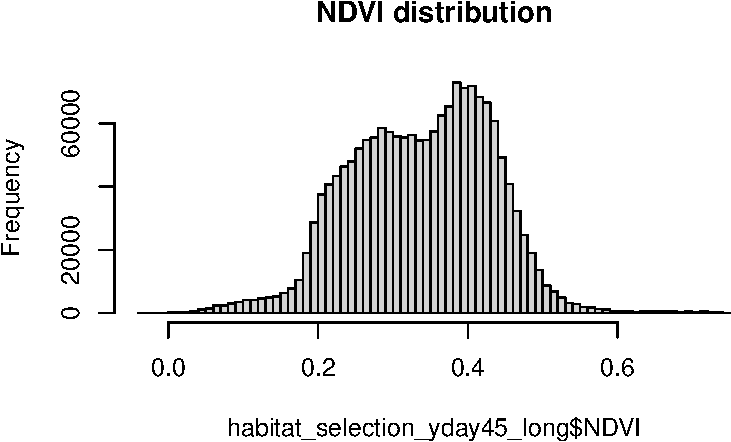
\includegraphics[keepaspectratio]{deepSSF_data_prep_id_files/figure-pdf/unnamed-chunk-5-1.pdf}}

\subsection{Read in the environmental
covariates}\label{read-in-the-environmental-covariates}

\begin{Shaded}
\begin{Highlighting}[]
\NormalTok{ndvi\_projected }\OtherTok{\textless{}{-}} \FunctionTok{rast}\NormalTok{(}\StringTok{"mapping/cropped rasters/ndvi\_GEE\_projected\_watermask20230207.tif"}\NormalTok{)}
\NormalTok{terra}\SpecialCharTok{::}\FunctionTok{time}\NormalTok{(ndvi\_projected) }\OtherTok{\textless{}{-}} \FunctionTok{as.POSIXct}\NormalTok{(lubridate}\SpecialCharTok{::}\FunctionTok{ymd}\NormalTok{(}\StringTok{"2018{-}01{-}01"}\NormalTok{) }\SpecialCharTok{+} \FunctionTok{months}\NormalTok{(}\DecValTok{0}\SpecialCharTok{:}\DecValTok{23}\NormalTok{))}
\NormalTok{slope }\OtherTok{\textless{}{-}} \FunctionTok{rast}\NormalTok{(}\StringTok{"mapping/cropped rasters/slope\_raster.tif"}\NormalTok{)}
\NormalTok{veg\_herby }\OtherTok{\textless{}{-}} \FunctionTok{rast}\NormalTok{(}\StringTok{"mapping/cropped rasters/veg\_herby.tif"}\NormalTok{)}
\NormalTok{canopy\_cover }\OtherTok{\textless{}{-}} \FunctionTok{rast}\NormalTok{(}\StringTok{"mapping/cropped rasters/canopy\_cover.tif"}\NormalTok{)}

\CommentTok{\# change the names (these will become the column names when extracting }
\CommentTok{\# covariate values at the used and random steps)}
\FunctionTok{names}\NormalTok{(ndvi\_projected) }\OtherTok{\textless{}{-}} \FunctionTok{rep}\NormalTok{(}\StringTok{"ndvi"}\NormalTok{, terra}\SpecialCharTok{::}\FunctionTok{nlyr}\NormalTok{(ndvi\_projected))}
\FunctionTok{names}\NormalTok{(slope) }\OtherTok{\textless{}{-}} \StringTok{"slope"}
\FunctionTok{names}\NormalTok{(veg\_herby) }\OtherTok{\textless{}{-}} \StringTok{"veg\_herby"}
\FunctionTok{names}\NormalTok{(canopy\_cover) }\OtherTok{\textless{}{-}} \StringTok{"canopy\_cover"}

\CommentTok{\# to plot the rasters}
\FunctionTok{plot}\NormalTok{(ndvi\_projected)}
\end{Highlighting}
\end{Shaded}

\pandocbounded{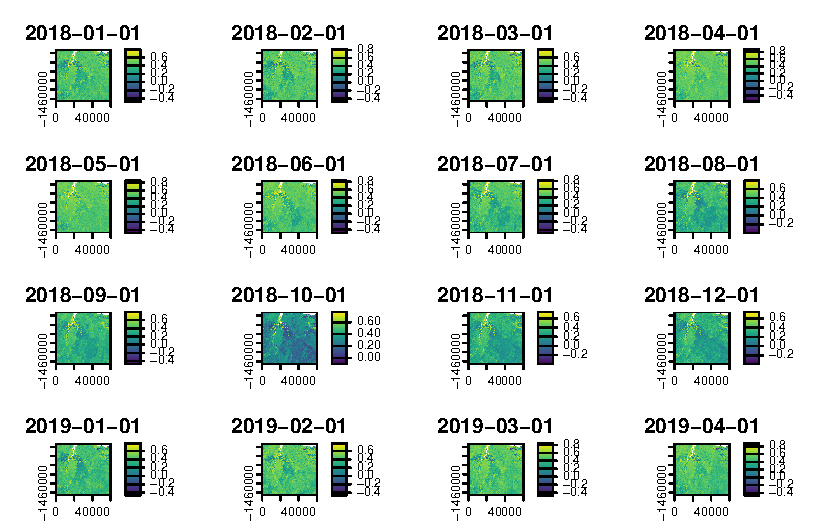
\includegraphics[keepaspectratio]{deepSSF_data_prep_id_files/figure-pdf/unnamed-chunk-6-1.pdf}}

\begin{Shaded}
\begin{Highlighting}[]
\FunctionTok{plot}\NormalTok{(ndvi\_projected[[}\DecValTok{1}\NormalTok{]])}
\end{Highlighting}
\end{Shaded}

\pandocbounded{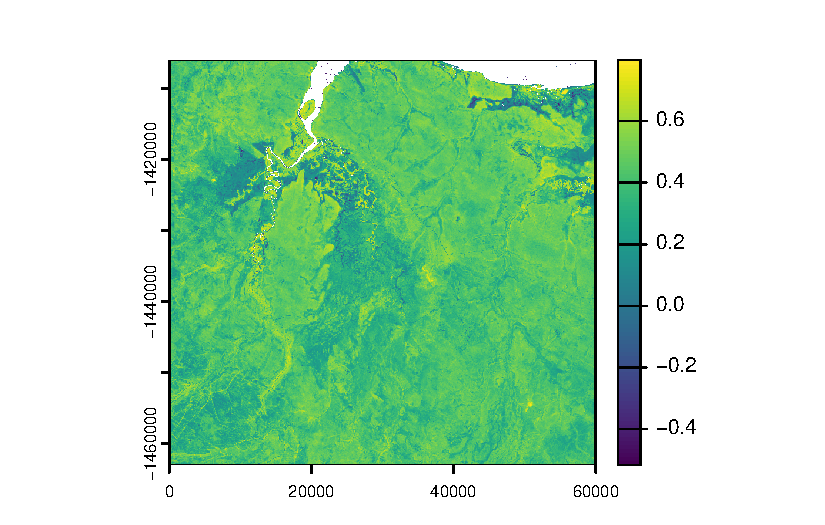
\includegraphics[keepaspectratio]{deepSSF_data_prep_id_files/figure-pdf/unnamed-chunk-6-2.pdf}}

\begin{Shaded}
\begin{Highlighting}[]
\FunctionTok{plot}\NormalTok{(slope)}
\end{Highlighting}
\end{Shaded}

\pandocbounded{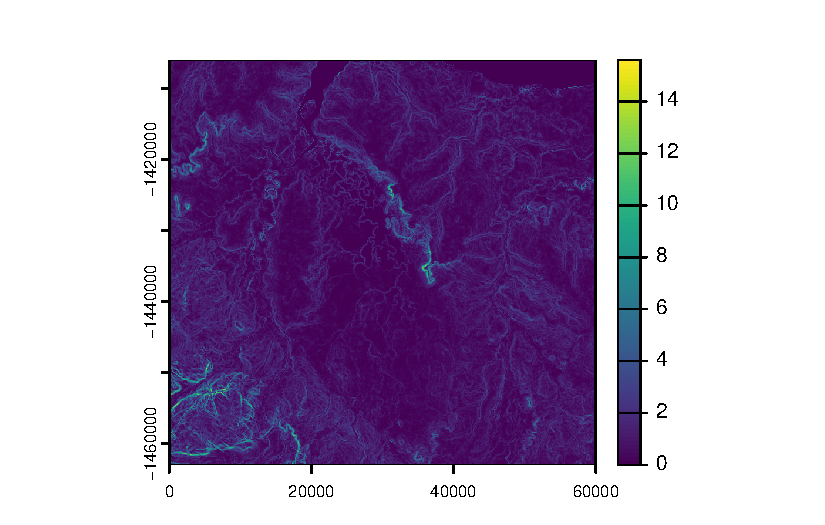
\includegraphics[keepaspectratio]{deepSSF_data_prep_id_files/figure-pdf/unnamed-chunk-6-3.pdf}}

\begin{Shaded}
\begin{Highlighting}[]
\FunctionTok{plot}\NormalTok{(veg\_herby)}
\end{Highlighting}
\end{Shaded}

\pandocbounded{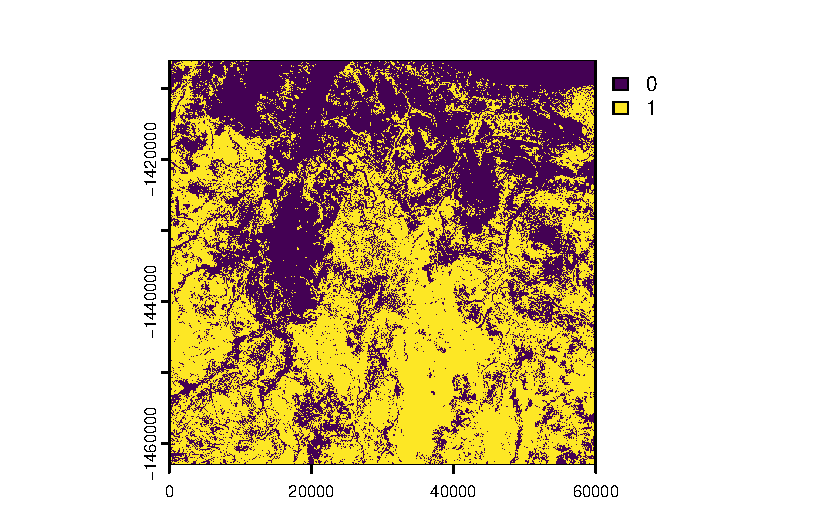
\includegraphics[keepaspectratio]{deepSSF_data_prep_id_files/figure-pdf/unnamed-chunk-6-4.pdf}}

\begin{Shaded}
\begin{Highlighting}[]
\FunctionTok{plot}\NormalTok{(canopy\_cover)}
\end{Highlighting}
\end{Shaded}

\pandocbounded{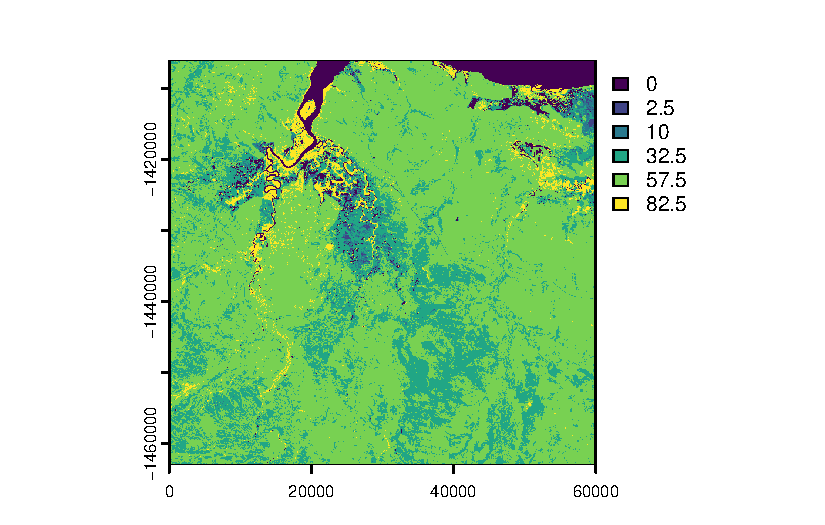
\includegraphics[keepaspectratio]{deepSSF_data_prep_id_files/figure-pdf/unnamed-chunk-6-5.pdf}}

\begin{Shaded}
\begin{Highlighting}[]
\CommentTok{\# get the resolution from the covariates}
\NormalTok{res }\OtherTok{\textless{}{-}}\NormalTok{ terra}\SpecialCharTok{::}\FunctionTok{res}\NormalTok{(ndvi\_projected)[}\DecValTok{1}\NormalTok{]}
\end{Highlighting}
\end{Shaded}

\section{Generating the data to fit a deepSSF
model}\label{generating-the-data-to-fit-a-deepssf-model}

\subsection{Create a steps object to check the step
lengths}\label{create-a-steps-object-to-check-the-step-lengths}

\begin{Shaded}
\begin{Highlighting}[]
\CommentTok{\# nest the data by individual}
\NormalTok{buffalo\_all\_nested }\OtherTok{\textless{}{-}}\NormalTok{ buffalo\_all }\SpecialCharTok{\%\textgreater{}\%} \FunctionTok{arrange}\NormalTok{(id) }\SpecialCharTok{\%\textgreater{}\%} \FunctionTok{nest}\NormalTok{(}\AttributeTok{data =} \SpecialCharTok{{-}}\StringTok{"id"}\NormalTok{)}

\NormalTok{buffalo\_all\_nested\_steps }\OtherTok{\textless{}{-}}\NormalTok{ buffalo\_all\_nested }\SpecialCharTok{\%\textgreater{}\%}
  \FunctionTok{mutate}\NormalTok{(}\AttributeTok{steps =} \FunctionTok{map}\NormalTok{(data, }\ControlFlowTok{function}\NormalTok{(x)}
\NormalTok{    x }\SpecialCharTok{\%\textgreater{}\%} 
      \CommentTok{\# track\_resample(rate = hours(1), tolerance = minutes(10)) \%\textgreater{}\%}
      \FunctionTok{steps}\NormalTok{()))}

\CommentTok{\# unnest the data after creating \textquotesingle{}steps\textquotesingle{} objects}
\NormalTok{buffalo\_all\_steps }\OtherTok{\textless{}{-}}\NormalTok{ buffalo\_all\_nested\_steps }\SpecialCharTok{\%\textgreater{}\%} 
\NormalTok{  amt}\SpecialCharTok{::}\FunctionTok{select}\NormalTok{(id, steps) }\SpecialCharTok{\%\textgreater{}\%} 
\NormalTok{  amt}\SpecialCharTok{::}\FunctionTok{unnest}\NormalTok{(}\AttributeTok{cols =}\NormalTok{ steps)}

\FunctionTok{head}\NormalTok{(buffalo\_all\_steps)}
\end{Highlighting}
\end{Shaded}

\begin{verbatim}
# A tibble: 6 x 11
  id       x1_    x2_       y1_       y2_   sl_ direction_p     ta_
* <chr>  <dbl>  <dbl>     <dbl>     <dbl> <dbl>       <dbl>   <dbl>
1 2005  41941. 41969. -1435875. -1435671. 206.        1.43  NA     
2 2005  41969. 41922. -1435671. -1435654.  50.7       2.80   1.37  
3 2005  41922. 41779. -1435654. -1435601. 152.        2.78  -0.0214
4 2005  41779. 41841. -1435601. -1435635.  70.7      -0.507  2.99  
5 2005  41841. 41655. -1435635. -1435604. 188.        2.98  -2.80  
6 2005  41655. 41619. -1435604. -1435608.  37.1      -3.02   0.285 
# i 3 more variables: t1_ <dttm>, t2_ <dttm>, dt_ <drtn>
\end{verbatim}

\subsubsection{Plot step lengths}\label{plot-step-lengths}

\begin{Shaded}
\begin{Highlighting}[]
\CommentTok{\# plot step lengths}
\NormalTok{buffalo\_all\_steps }\SpecialCharTok{\%\textgreater{}\%} 
  \FunctionTok{filter}\NormalTok{(sl\_ }\SpecialCharTok{\textless{}} \DecValTok{2000}\NormalTok{) }\SpecialCharTok{\%\textgreater{}\%}
  \FunctionTok{ggplot}\NormalTok{() }\SpecialCharTok{+}
  \FunctionTok{geom\_density}\NormalTok{(}\FunctionTok{aes}\NormalTok{(}\AttributeTok{x =}\NormalTok{ sl\_), }\CommentTok{\#, bins = 50}
                 \AttributeTok{fill =} \StringTok{"skyblue"}\NormalTok{, }\AttributeTok{colour =} \StringTok{"skyblue"}\NormalTok{, }\AttributeTok{alpha =} \FloatTok{0.75}\NormalTok{) }\SpecialCharTok{+}
  \FunctionTok{scale\_x\_continuous}\NormalTok{(}\StringTok{"Step length (m)"}\NormalTok{) }\SpecialCharTok{+} \CommentTok{\#, limits = c({-}25, 1250)}
  \FunctionTok{scale\_y\_continuous}\NormalTok{(}\StringTok{"Density"}\NormalTok{) }\SpecialCharTok{+}
  \FunctionTok{ggtitle}\NormalTok{(}\StringTok{"Step lengths"}\NormalTok{) }\SpecialCharTok{+}
  \FunctionTok{theme\_classic}\NormalTok{()}
\end{Highlighting}
\end{Shaded}

\pandocbounded{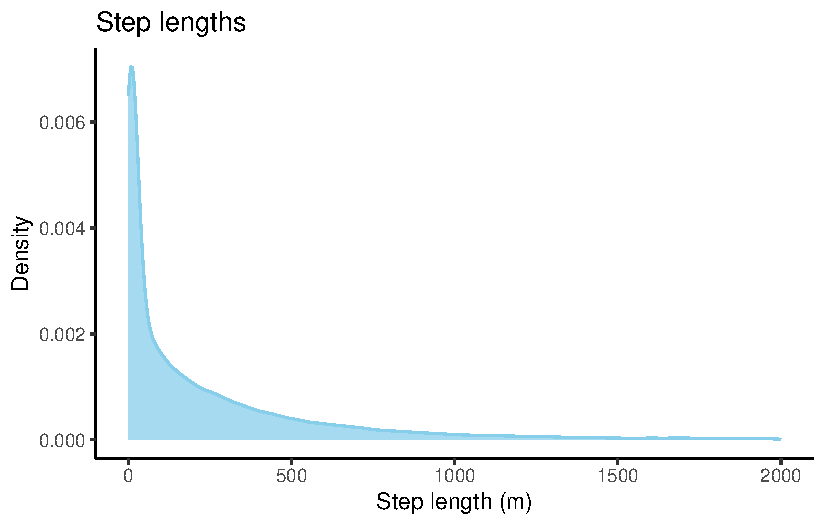
\includegraphics[keepaspectratio]{deepSSF_data_prep_id_files/figure-pdf/unnamed-chunk-8-1.pdf}}

\begin{Shaded}
\begin{Highlighting}[]
\CommentTok{\# proportion of steps less than the buffer distance}
\CommentTok{\# the distance should be a multiple of the resolution}
\NormalTok{distance }\OtherTok{\textless{}{-}} \DecValTok{1250}

\CommentTok{\# check if multiple of the resolution?}
\NormalTok{distance }\SpecialCharTok{\%\%}\NormalTok{ res }\SpecialCharTok{==} \DecValTok{0}
\end{Highlighting}
\end{Shaded}

\begin{verbatim}
[1] TRUE
\end{verbatim}

\begin{Shaded}
\begin{Highlighting}[]
\CommentTok{\# buffer distance (add the resolution of the cell/2 as we want a centre cell)}
\NormalTok{buffer }\OtherTok{\textless{}{-}} \DecValTok{1250} \SpecialCharTok{+}\NormalTok{ (res}\SpecialCharTok{/}\DecValTok{2}\NormalTok{)}

\CommentTok{\# calculate proportion}
\NormalTok{prop\_steps }\OtherTok{\textless{}{-}}\NormalTok{ buffalo\_all\_steps }\SpecialCharTok{\%\textgreater{}\%} \FunctionTok{filter}\NormalTok{(sl\_ }\SpecialCharTok{\textless{}}\NormalTok{ buffer) }\SpecialCharTok{\%\textgreater{}\%} \FunctionTok{nrow}\NormalTok{() }\SpecialCharTok{/}\NormalTok{ buffalo\_all\_steps }\SpecialCharTok{\%\textgreater{}\%} \FunctionTok{nrow}\NormalTok{()}
\FunctionTok{print}\NormalTok{(}\FunctionTok{paste0}\NormalTok{(}\StringTok{"Proportion of steps less than "}\NormalTok{, buffer, }\StringTok{"m: "}\NormalTok{, }\FunctionTok{round}\NormalTok{(prop\_steps, }\DecValTok{4}\NormalTok{)))}
\end{Highlighting}
\end{Shaded}

\begin{verbatim}
[1] "Proportion of steps less than 1262.5m: 0.9573"
\end{verbatim}

\begin{Shaded}
\begin{Highlighting}[]
\CommentTok{\# distance to the corner}
\NormalTok{corner\_dist }\OtherTok{\textless{}{-}} \FunctionTok{sqrt}\NormalTok{(buffer}\SpecialCharTok{\^{}}\DecValTok{2} \SpecialCharTok{+}\NormalTok{ buffer}\SpecialCharTok{\^{}}\DecValTok{2}\NormalTok{)}
\FunctionTok{print}\NormalTok{(}\FunctionTok{paste0}\NormalTok{(}\StringTok{"Distance to the corner: "}\NormalTok{, }\FunctionTok{round}\NormalTok{(corner\_dist, }\DecValTok{2}\NormalTok{)))}
\end{Highlighting}
\end{Shaded}

\begin{verbatim}
[1] "Distance to the corner: 1785.44"
\end{verbatim}

In our case 95\% of the steps were less than a distance of 1262.5m,
which would mean that including 101 x 101 cells (which would be 2525 m x
2525 m) would include at least 95\% of the steps.

Note: as 1262.5 m is the shortest distance to the boundary, and it is
further to a corner (which is 1786 m away), which means we will actually
be including more than 95\% of the steps.

\subsection{Set up the spatial extent of the local
covariates}\label{set-up-the-spatial-extent-of-the-local-covariates}

We calculate the number of cells in each axis, and set the lag between
locations. Typically this will just be 1, as we want the next-step to be
the target. However, it may be possible to improve model training by
using different lags and including the time difference between locations
as a covariate. I expect that this would help to predict across
different time scales and not be restricted to the time scale that the
data was collected at.

\begin{Shaded}
\begin{Highlighting}[]
\CommentTok{\# calculate the number of cells in each axis}
\NormalTok{nxn\_cells }\OtherTok{\textless{}{-}}\NormalTok{ buffer}\SpecialCharTok{*}\DecValTok{2}\SpecialCharTok{/}\NormalTok{res}
\FunctionTok{print}\NormalTok{(}\FunctionTok{paste0}\NormalTok{(}\StringTok{"Number of cells in each axis: "}\NormalTok{, nxn\_cells))}
\end{Highlighting}
\end{Shaded}

\begin{verbatim}
[1] "Number of cells in each axis: 101"
\end{verbatim}

\begin{Shaded}
\begin{Highlighting}[]
\CommentTok{\# hourly lag {-} to set larger time differences between locations}
\NormalTok{hourly\_lag }\OtherTok{\textless{}{-}} \DecValTok{1}
\end{Highlighting}
\end{Shaded}

\section{Loop over each individual and save the local
rasters}\label{loop-over-each-individual-and-save-the-local-rasters}

This is the main function of the script. It loops over each individual
and calculates step level information, such as the location and time of
the next step (x2, y2, t2), step length, turning angle, and different
time components.

It also determines where to crop the local layers by subtracting and
adding the buffer distance from the location of each step. It then crops
out the local layers for each step and saves them as a list entry into
the data frame.

It then creates a raster stack (with the number of layers equal to the
number of steps) for each covariate and saves it as a tif.

For each individual, this will therefore create a csv containing the
step level information, and a tif for each covariate containing the
local layers for each step.

It takes quite a while to run, around 1 hour per individual in our case,
so we will illustrate the function with 10 steps per individual.
Uncomment the line specified in the loop to use the full dataset.

\begin{Shaded}
\begin{Highlighting}[]
\ControlFlowTok{for}\NormalTok{(i }\ControlFlowTok{in} \DecValTok{1}\SpecialCharTok{:}\FunctionTok{length}\NormalTok{(buffalo\_ids)) \{}

\NormalTok{  buffalo\_data }\OtherTok{\textless{}{-}}\NormalTok{ buffalo\_all }\SpecialCharTok{\%\textgreater{}\%} \FunctionTok{filter}\NormalTok{(id }\SpecialCharTok{==}\NormalTok{ buffalo\_ids[i])}
  \CommentTok{\# all data for that individual}
\NormalTok{  buffalo\_data }\OtherTok{\textless{}{-}}\NormalTok{ buffalo\_data }\SpecialCharTok{\%\textgreater{}\%} \FunctionTok{arrange}\NormalTok{(t\_)}
  
  \CommentTok{\# to use a subset of the data for that individual for testing}
  \CommentTok{\# COMMENT THIS LINE OUT TO USE THE FULL DATASET}
\NormalTok{  buffalo\_data }\OtherTok{\textless{}{-}}\NormalTok{ buffalo\_data }\SpecialCharTok{\%\textgreater{}\%} \FunctionTok{arrange}\NormalTok{(t\_) }\SpecialCharTok{|\textgreater{}}  \FunctionTok{slice}\NormalTok{(}\DecValTok{1}\SpecialCharTok{:}\DecValTok{100}\NormalTok{)}

\NormalTok{  n\_samples }\OtherTok{\textless{}{-}} \FunctionTok{nrow}\NormalTok{(buffalo\_data)}
  
  \FunctionTok{tic}\NormalTok{()}
  
\NormalTok{  buffalo\_data\_covs }\OtherTok{\textless{}{-}}\NormalTok{ buffalo\_data }\SpecialCharTok{\%\textgreater{}\%} \FunctionTok{mutate}\NormalTok{(}
    
    \AttributeTok{x1\_ =}\NormalTok{ x\_,}
    \AttributeTok{y1\_ =}\NormalTok{ y\_,}
    \AttributeTok{x2\_ =} \FunctionTok{lead}\NormalTok{(x1\_, }\AttributeTok{n =}\NormalTok{ hourly\_lag, }\AttributeTok{default =} \ConstantTok{NA}\NormalTok{),}
    \AttributeTok{y2\_ =} \FunctionTok{lead}\NormalTok{(y1\_, }\AttributeTok{n =}\NormalTok{ hourly\_lag, }\AttributeTok{default =} \ConstantTok{NA}\NormalTok{),}
    \AttributeTok{x2\_cent =}\NormalTok{ x2\_ }\SpecialCharTok{{-}}\NormalTok{ x1\_,}
    \AttributeTok{y2\_cent =}\NormalTok{ y2\_ }\SpecialCharTok{{-}}\NormalTok{ y1\_,}
    \AttributeTok{t2\_ =} \FunctionTok{lead}\NormalTok{(t\_, }\AttributeTok{n =}\NormalTok{ hourly\_lag, }\AttributeTok{default =} \ConstantTok{NA}\NormalTok{),}
    \AttributeTok{t\_diff =} \FunctionTok{round}\NormalTok{(}\FunctionTok{difftime}\NormalTok{(t2\_, t\_, }\AttributeTok{units =} \StringTok{"hours"}\NormalTok{),}\DecValTok{0}\NormalTok{),}
    \AttributeTok{hour\_t1 =}\NormalTok{ lubridate}\SpecialCharTok{::}\FunctionTok{hour}\NormalTok{(t\_),}
    \AttributeTok{yday\_t1 =}\NormalTok{ lubridate}\SpecialCharTok{::}\FunctionTok{yday}\NormalTok{(t\_),}
    \AttributeTok{hour\_t2 =}\NormalTok{ lubridate}\SpecialCharTok{::}\FunctionTok{hour}\NormalTok{(t2\_),}
    \AttributeTok{hour\_t2\_sin =} \FunctionTok{sin}\NormalTok{(}\DecValTok{2}\SpecialCharTok{*}\NormalTok{pi}\SpecialCharTok{*}\NormalTok{hour\_t2}\SpecialCharTok{/}\DecValTok{24}\NormalTok{),}
    \AttributeTok{hour\_t2\_cos =} \FunctionTok{cos}\NormalTok{(}\DecValTok{2}\SpecialCharTok{*}\NormalTok{pi}\SpecialCharTok{*}\NormalTok{hour\_t2}\SpecialCharTok{/}\DecValTok{24}\NormalTok{),}
    \AttributeTok{yday\_t2 =}\NormalTok{ lubridate}\SpecialCharTok{::}\FunctionTok{yday}\NormalTok{(t2\_),}
    \AttributeTok{yday\_t2\_sin =} \FunctionTok{sin}\NormalTok{(}\DecValTok{2}\SpecialCharTok{*}\NormalTok{pi}\SpecialCharTok{*}\NormalTok{yday\_t2}\SpecialCharTok{/}\FloatTok{365.25}\NormalTok{),}
    \AttributeTok{yday\_t2\_cos =} \FunctionTok{cos}\NormalTok{(}\DecValTok{2}\SpecialCharTok{*}\NormalTok{pi}\SpecialCharTok{*}\NormalTok{yday\_t2}\SpecialCharTok{/}\FloatTok{365.25}\NormalTok{),}
    
    \AttributeTok{sl =} \FunctionTok{c}\NormalTok{(}\FunctionTok{sqrt}\NormalTok{(}\FunctionTok{diff}\NormalTok{(y\_)}\SpecialCharTok{\^{}}\DecValTok{2} \SpecialCharTok{+} \FunctionTok{diff}\NormalTok{(x\_)}\SpecialCharTok{\^{}}\DecValTok{2}\NormalTok{), }\ConstantTok{NA}\NormalTok{),}
    \AttributeTok{log\_sl =} \FunctionTok{log}\NormalTok{(sl),}
    \AttributeTok{bearing =} \FunctionTok{c}\NormalTok{(}\FunctionTok{atan2}\NormalTok{(}\FunctionTok{diff}\NormalTok{(y\_), }\FunctionTok{diff}\NormalTok{(x\_)), }\ConstantTok{NA}\NormalTok{),}
    \AttributeTok{bearing\_sin =} \FunctionTok{sin}\NormalTok{(bearing),}
    \AttributeTok{bearing\_cos =} \FunctionTok{cos}\NormalTok{(bearing),}
    \AttributeTok{ta =} \FunctionTok{c}\NormalTok{(}\ConstantTok{NA}\NormalTok{, }\FunctionTok{ifelse}\NormalTok{(}
      \FunctionTok{diff}\NormalTok{(bearing) }\SpecialCharTok{\textgreater{}}\NormalTok{ pi, }\FunctionTok{diff}\NormalTok{(bearing)}\SpecialCharTok{{-}}\NormalTok{(}\DecValTok{2}\SpecialCharTok{*}\NormalTok{pi), }\FunctionTok{ifelse}\NormalTok{(}
        \FunctionTok{diff}\NormalTok{(bearing) }\SpecialCharTok{\textless{}} \SpecialCharTok{{-}}\NormalTok{pi, }\FunctionTok{diff}\NormalTok{(bearing)}\SpecialCharTok{+}\NormalTok{(}\DecValTok{2}\SpecialCharTok{*}\NormalTok{pi), }\FunctionTok{diff}\NormalTok{(bearing)))),}
    \AttributeTok{cos\_ta =} \FunctionTok{cos}\NormalTok{(ta),}
      
    \CommentTok{\# extent for cropping the spatial covariates}
    \AttributeTok{x\_min =}\NormalTok{ x\_ }\SpecialCharTok{{-}}\NormalTok{ buffer,}
    \AttributeTok{x\_max =}\NormalTok{ x\_ }\SpecialCharTok{+}\NormalTok{ buffer,}
    \AttributeTok{y\_min =}\NormalTok{ y\_ }\SpecialCharTok{{-}}\NormalTok{ buffer,}
    \AttributeTok{y\_max =}\NormalTok{ y\_ }\SpecialCharTok{+}\NormalTok{ buffer,}
    
  
    \CommentTok{\# crop out and store the local covariates centered on the animal\textquotesingle{}s location }
    \CommentTok{\# with an extent set in the previous chunk}
\NormalTok{  ) }\SpecialCharTok{\%\textgreater{}\%} \FunctionTok{rowwise}\NormalTok{() }\SpecialCharTok{\%\textgreater{}\%} \FunctionTok{mutate}\NormalTok{(}

    \AttributeTok{extent\_00centre =} \FunctionTok{list}\NormalTok{(}\FunctionTok{ext}\NormalTok{(x\_min }\SpecialCharTok{{-}}\NormalTok{ x\_, x\_max }\SpecialCharTok{{-}}\NormalTok{ x\_, y\_min }\SpecialCharTok{{-}}\NormalTok{ y\_, y\_max }\SpecialCharTok{{-}}\NormalTok{ y\_)),}

    \CommentTok{\# NDVI}
    \AttributeTok{ndvi\_index =} \FunctionTok{which.min}\NormalTok{(}\FunctionTok{abs}\NormalTok{(}\FunctionTok{difftime}\NormalTok{(t\_, terra}\SpecialCharTok{::}\FunctionTok{time}\NormalTok{(ndvi\_projected)))),}
    \AttributeTok{ndvi\_cent =} \FunctionTok{list}\NormalTok{(\{}
\NormalTok{      ndvi\_cent }\OtherTok{=} \FunctionTok{crop}\NormalTok{(ndvi\_projected[[ndvi\_index]], }\FunctionTok{ext}\NormalTok{(x\_min, x\_max, y\_min, y\_max))}
      \FunctionTok{ext}\NormalTok{(ndvi\_cent) }\OtherTok{\textless{}{-}}\NormalTok{ extent\_00centre}
\NormalTok{      ndvi\_cent}
\NormalTok{      \}),}

    \CommentTok{\# herbaceous vegetation}
    \AttributeTok{veg\_herby\_cent =} \FunctionTok{list}\NormalTok{(\{}
\NormalTok{      veg\_herby\_cent }\OtherTok{=} \FunctionTok{crop}\NormalTok{(veg\_herby, }\FunctionTok{ext}\NormalTok{(x\_min, x\_max, y\_min, y\_max))}
      \FunctionTok{ext}\NormalTok{(veg\_herby\_cent) }\OtherTok{\textless{}{-}}\NormalTok{ extent\_00centre}
\NormalTok{      veg\_herby\_cent}
\NormalTok{      \}),}

    \CommentTok{\# canopy cover}
    \AttributeTok{canopy\_cover\_cent =} \FunctionTok{list}\NormalTok{(\{}
\NormalTok{      canopy\_cover\_cent }\OtherTok{=} \FunctionTok{crop}\NormalTok{(canopy\_cover, }\FunctionTok{ext}\NormalTok{(x\_min, x\_max, y\_min, y\_max))}
      \FunctionTok{ext}\NormalTok{(canopy\_cover\_cent) }\OtherTok{\textless{}{-}}\NormalTok{ extent\_00centre}
\NormalTok{      canopy\_cover\_cent}
\NormalTok{      \}),}

    \CommentTok{\# slope}
    \AttributeTok{slope\_cent =} \FunctionTok{list}\NormalTok{(\{}
\NormalTok{      slope\_cent }\OtherTok{\textless{}{-}} \FunctionTok{crop}\NormalTok{(slope, }\FunctionTok{ext}\NormalTok{(x\_min, x\_max, y\_min, y\_max))}
      \FunctionTok{ext}\NormalTok{(slope\_cent) }\OtherTok{\textless{}{-}}\NormalTok{ extent\_00centre}
\NormalTok{      slope\_cent}
\NormalTok{      \}),}

    \CommentTok{\# rasterised location of the next step {-} centred on (0,0)}
    \AttributeTok{points\_vect\_cent =} \FunctionTok{list}\NormalTok{(terra}\SpecialCharTok{::}\FunctionTok{vect}\NormalTok{(}\FunctionTok{cbind}\NormalTok{(x2\_ }\SpecialCharTok{{-}}\NormalTok{ x\_, y2\_ }\SpecialCharTok{{-}}\NormalTok{ y\_), }\AttributeTok{type =} \StringTok{"points"}\NormalTok{, }\AttributeTok{crs =} \StringTok{"EPSG:3112"}\NormalTok{)),}
    \AttributeTok{pres\_cent =} \FunctionTok{list}\NormalTok{(}\FunctionTok{rasterize}\NormalTok{(points\_vect\_cent, ndvi\_cent, }\AttributeTok{background=}\DecValTok{0}\NormalTok{))}

\NormalTok{  ) }\SpecialCharTok{\%\textgreater{}\%} \FunctionTok{ungroup}\NormalTok{() }\CommentTok{\# to remove the \textquotesingle{}rowwise\textquotesingle{} class}


  \FunctionTok{toc}\NormalTok{()}

  \CommentTok{\# remove steps that fall outside of the local spatial extent}
\NormalTok{  buffalo\_data\_covs }\OtherTok{\textless{}{-}}\NormalTok{ buffalo\_data\_covs }\SpecialCharTok{\%\textgreater{}\%}
    \FunctionTok{filter}\NormalTok{(x2\_cent }\SpecialCharTok{\textgreater{}} \SpecialCharTok{{-}}\NormalTok{buffer }\SpecialCharTok{\&}\NormalTok{ x2\_cent }\SpecialCharTok{\textless{}}\NormalTok{ buffer }\SpecialCharTok{\&}\NormalTok{ y2\_cent }\SpecialCharTok{\textgreater{}} \SpecialCharTok{{-}}\NormalTok{buffer }\SpecialCharTok{\&}\NormalTok{ y2\_cent }\SpecialCharTok{\textless{}}\NormalTok{ buffer) }\SpecialCharTok{\%\textgreater{}\%}
    \FunctionTok{drop\_na}\NormalTok{(ta)}

  \CommentTok{\# remove the columns that are no longer needed}
\NormalTok{  buffalo\_data\_df }\OtherTok{\textless{}{-}}\NormalTok{ buffalo\_data\_covs }\SpecialCharTok{\%\textgreater{}\%}
\NormalTok{  dplyr}\SpecialCharTok{::}\FunctionTok{select}\NormalTok{(}\SpecialCharTok{{-}}\NormalTok{extent\_00centre,}
                \SpecialCharTok{{-}}\NormalTok{ndvi\_cent,}
                \SpecialCharTok{{-}}\NormalTok{veg\_herby\_cent,}
                \SpecialCharTok{{-}}\NormalTok{canopy\_cover\_cent,}
                \SpecialCharTok{{-}}\NormalTok{slope\_cent,}
                \SpecialCharTok{{-}}\NormalTok{points\_vect\_cent,}
                \SpecialCharTok{{-}}\NormalTok{pres\_cent}
\NormalTok{                )}

  \CommentTok{\# save the data}
  \FunctionTok{write\_csv}\NormalTok{(buffalo\_data\_df, }\FunctionTok{paste0}\NormalTok{(}\StringTok{"buffalo\_local\_data\_id/buffalo\_"}\NormalTok{, buffalo\_ids[i],}
                                    \StringTok{"\_data\_df\_lag\_"}\NormalTok{, hourly\_lag, }\StringTok{"hr\_n"}\NormalTok{, n\_samples, }\StringTok{".csv"}\NormalTok{))}

  \CommentTok{\# saving the raster objects}
  \FunctionTok{rast}\NormalTok{(buffalo\_data\_covs}\SpecialCharTok{$}\NormalTok{ndvi\_cent) }\SpecialCharTok{\%\textgreater{}\%}
    \FunctionTok{writeRaster}\NormalTok{(}\FunctionTok{paste0}\NormalTok{(}\StringTok{"buffalo\_local\_layers\_id/buffalo\_"}\NormalTok{, buffalo\_ids[i], }\StringTok{"\_ndvi\_cent"}\NormalTok{,}
\NormalTok{                       nxn\_cells, }\StringTok{"x"}\NormalTok{, nxn\_cells, }\StringTok{"\_lag\_"}\NormalTok{, hourly\_lag, }\StringTok{"hr\_n"}\NormalTok{, n\_samples, }\StringTok{".tif"}\NormalTok{),}
                \AttributeTok{overwrite =}\NormalTok{ T)}

  \FunctionTok{rast}\NormalTok{(buffalo\_data\_covs}\SpecialCharTok{$}\NormalTok{veg\_herby\_cent) }\SpecialCharTok{\%\textgreater{}\%}
    \FunctionTok{writeRaster}\NormalTok{(}\FunctionTok{paste0}\NormalTok{(}\StringTok{"buffalo\_local\_layers\_id/buffalo\_"}\NormalTok{, buffalo\_ids[i], }\StringTok{"\_herby\_cent"}\NormalTok{,}
\NormalTok{                       nxn\_cells, }\StringTok{"x"}\NormalTok{, nxn\_cells, }\StringTok{"\_lag\_"}\NormalTok{, hourly\_lag, }\StringTok{"hr\_n"}\NormalTok{, n\_samples, }\StringTok{".tif"}\NormalTok{),}
                \AttributeTok{overwrite =}\NormalTok{ T)}

  \FunctionTok{rast}\NormalTok{(buffalo\_data\_covs}\SpecialCharTok{$}\NormalTok{canopy\_cover\_cent) }\SpecialCharTok{\%\textgreater{}\%}
    \FunctionTok{writeRaster}\NormalTok{(}\FunctionTok{paste0}\NormalTok{(}\StringTok{"buffalo\_local\_layers\_id/buffalo\_"}\NormalTok{, buffalo\_ids[i], }\StringTok{"\_canopy\_cent"}\NormalTok{,}
\NormalTok{                       nxn\_cells, }\StringTok{"x"}\NormalTok{, nxn\_cells, }\StringTok{"\_lag\_"}\NormalTok{, hourly\_lag, }\StringTok{"hr\_n"}\NormalTok{, n\_samples, }\StringTok{".tif"}\NormalTok{),}
                \AttributeTok{overwrite =}\NormalTok{ T)}

  \FunctionTok{rast}\NormalTok{(buffalo\_data\_covs}\SpecialCharTok{$}\NormalTok{slope\_cent) }\SpecialCharTok{\%\textgreater{}\%}
    \FunctionTok{writeRaster}\NormalTok{(}\FunctionTok{paste0}\NormalTok{(}\StringTok{"buffalo\_local\_layers\_id/buffalo\_"}\NormalTok{, buffalo\_ids[i], }\StringTok{"\_slope\_cent"}\NormalTok{,}
\NormalTok{                       nxn\_cells, }\StringTok{"x"}\NormalTok{, nxn\_cells, }\StringTok{"\_lag\_"}\NormalTok{, hourly\_lag, }\StringTok{"hr\_n"}\NormalTok{, n\_samples, }\StringTok{".tif"}\NormalTok{),}
                \AttributeTok{overwrite =}\NormalTok{ T)}

  \FunctionTok{rast}\NormalTok{(buffalo\_data\_covs}\SpecialCharTok{$}\NormalTok{pres\_cent) }\SpecialCharTok{\%\textgreater{}\%}
    \FunctionTok{writeRaster}\NormalTok{(}\FunctionTok{paste0}\NormalTok{(}\StringTok{"buffalo\_local\_layers\_id/buffalo\_"}\NormalTok{, buffalo\_ids[i], }\StringTok{"\_pres\_cent"}\NormalTok{,}
\NormalTok{                       nxn\_cells, }\StringTok{"x"}\NormalTok{, nxn\_cells, }\StringTok{"\_lag\_"}\NormalTok{, hourly\_lag, }\StringTok{"hr\_n"}\NormalTok{, n\_samples, }\StringTok{".tif"}\NormalTok{),}
                \AttributeTok{overwrite =}\NormalTok{ T)}
  
\NormalTok{\}}
\end{Highlighting}
\end{Shaded}

\begin{verbatim}
22.64 sec elapsed
18.69 sec elapsed
19.85 sec elapsed
19.99 sec elapsed
21.54 sec elapsed
24.54 sec elapsed
20.83 sec elapsed
22.34 sec elapsed
20.75 sec elapsed
26.36 sec elapsed
22.33 sec elapsed
18.09 sec elapsed
13.9 sec elapsed
\end{verbatim}

\subsection{Check the outputs}\label{check-the-outputs}

\begin{Shaded}
\begin{Highlighting}[]
\FunctionTok{head}\NormalTok{(buffalo\_data\_covs)}
\end{Highlighting}
\end{Shaded}

\begin{verbatim}
# A tibble: 6 x 39
      x_      y_ t_                  id       x1_     y1_    x2_     y2_ x2_cent
   <dbl>   <dbl> <dttm>              <chr>  <dbl>   <dbl>  <dbl>   <dbl>   <dbl>
1 32550. -1.42e6 2018-07-25 12:11:31 2393  32550. -1.42e6 32551. -1.42e6   0.323
2 32551. -1.42e6 2018-07-25 13:10:28 2393  32551. -1.42e6 32550. -1.42e6  -1.13 
3 32550. -1.42e6 2018-07-25 14:11:04 2393  32550. -1.42e6 32552. -1.42e6   2.57 
4 32552. -1.42e6 2018-07-25 15:12:01 2393  32552. -1.42e6 32556. -1.42e6   3.67 
5 32556. -1.42e6 2018-07-25 16:10:49 2393  32556. -1.42e6 32551. -1.42e6  -4.85 
6 32551. -1.42e6 2018-07-25 17:12:20 2393  32551. -1.42e6 32547. -1.42e6  -4.18 
# i 30 more variables: y2_cent <dbl>, t2_ <dttm>, t_diff <drtn>, hour_t1 <int>,
#   yday_t1 <dbl>, hour_t2 <int>, hour_t2_sin <dbl>, hour_t2_cos <dbl>,
#   yday_t2 <dbl>, yday_t2_sin <dbl>, yday_t2_cos <dbl>, sl <dbl>,
#   log_sl <dbl>, bearing <dbl>, bearing_sin <dbl>, bearing_cos <dbl>,
#   ta <dbl>, cos_ta <dbl>, x_min <dbl>, x_max <dbl>, y_min <dbl>, y_max <dbl>,
#   extent_00centre <list>, ndvi_index <int>, ndvi_cent <list>,
#   veg_herby_cent <list>, canopy_cover_cent <list>, slope_cent <list>, ...
\end{verbatim}

\begin{Shaded}
\begin{Highlighting}[]
\FunctionTok{which}\NormalTok{(}\FunctionTok{is.na}\NormalTok{(buffalo\_data\_covs}\SpecialCharTok{$}\NormalTok{ta))}
\end{Highlighting}
\end{Shaded}

\begin{verbatim}
integer(0)
\end{verbatim}

\subsection{Plot a subset of the local
covariates}\label{plot-a-subset-of-the-local-covariates}

\begin{Shaded}
\begin{Highlighting}[]
\NormalTok{n\_plots }\OtherTok{\textless{}{-}} \DecValTok{3}

\CommentTok{\# NDVI}
\FunctionTok{walk}\NormalTok{(buffalo\_data\_covs}\SpecialCharTok{$}\NormalTok{ndvi\_cent[}\DecValTok{1}\SpecialCharTok{:}\NormalTok{n\_plots], terra}\SpecialCharTok{::}\NormalTok{plot)}
\end{Highlighting}
\end{Shaded}

\pandocbounded{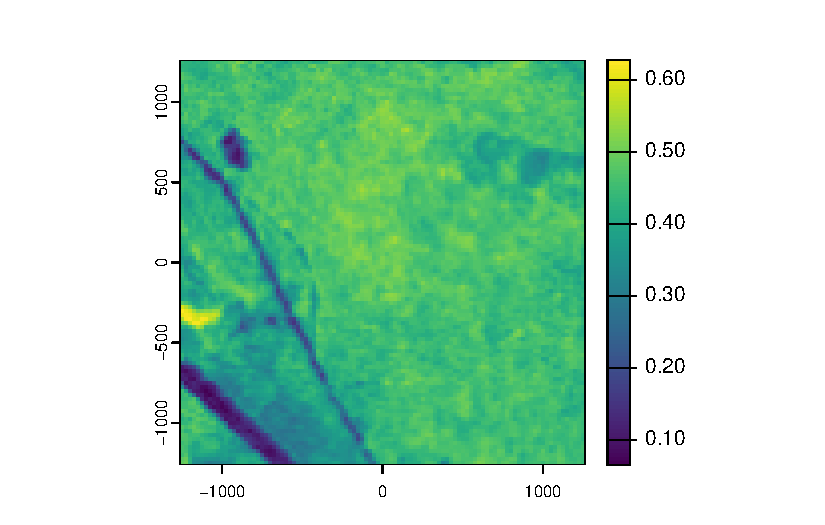
\includegraphics[keepaspectratio]{deepSSF_data_prep_id_files/figure-pdf/unnamed-chunk-12-1.pdf}}

\pandocbounded{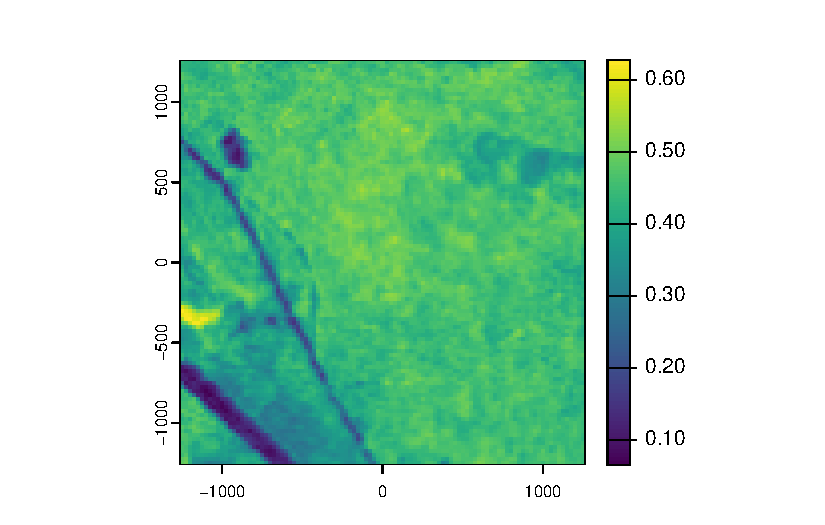
\includegraphics[keepaspectratio]{deepSSF_data_prep_id_files/figure-pdf/unnamed-chunk-12-2.pdf}}

\pandocbounded{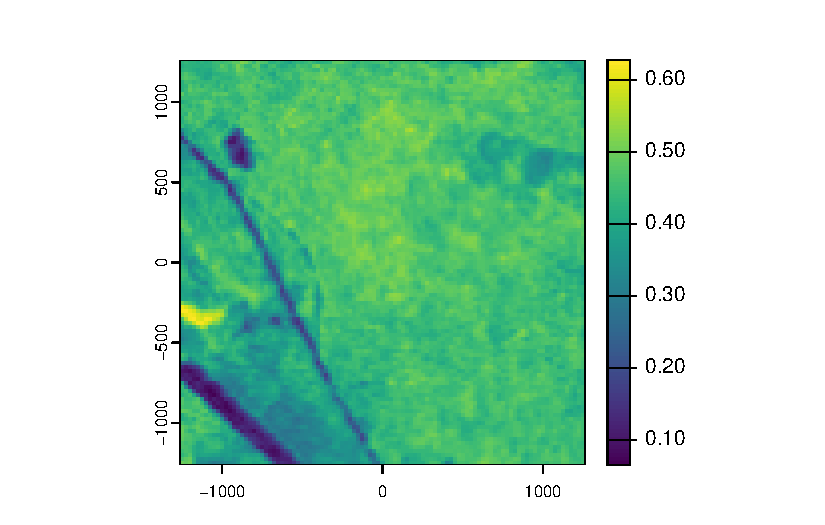
\includegraphics[keepaspectratio]{deepSSF_data_prep_id_files/figure-pdf/unnamed-chunk-12-3.pdf}}

\begin{Shaded}
\begin{Highlighting}[]
\CommentTok{\# Herbaceous vegetation}
\FunctionTok{walk}\NormalTok{(buffalo\_data\_covs}\SpecialCharTok{$}\NormalTok{veg\_herby\_cent[}\DecValTok{1}\SpecialCharTok{:}\NormalTok{n\_plots], terra}\SpecialCharTok{::}\NormalTok{plot)}
\end{Highlighting}
\end{Shaded}

\pandocbounded{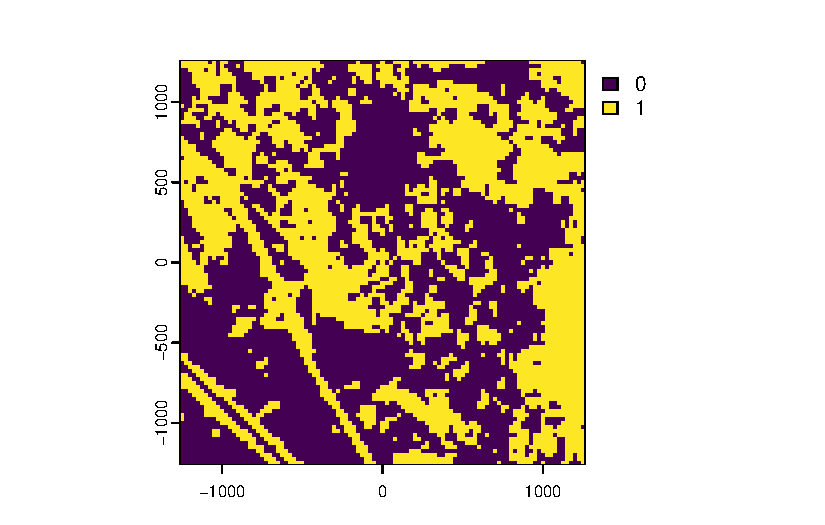
\includegraphics[keepaspectratio]{deepSSF_data_prep_id_files/figure-pdf/unnamed-chunk-12-4.pdf}}

\pandocbounded{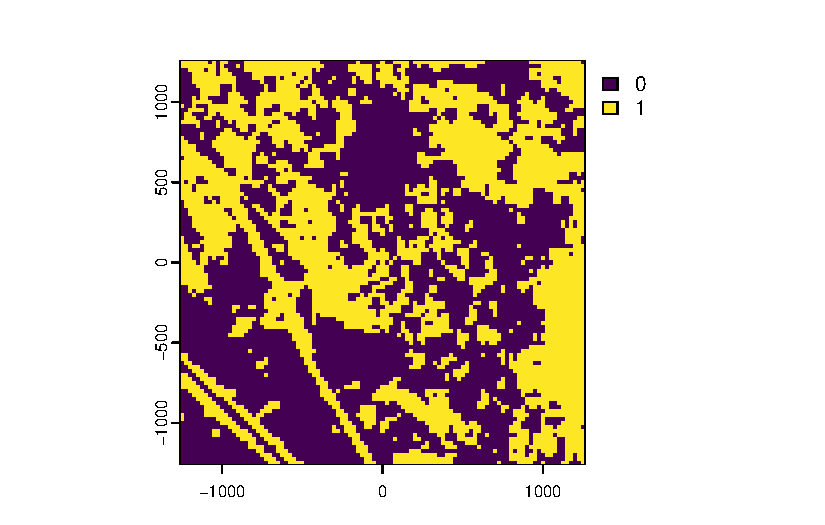
\includegraphics[keepaspectratio]{deepSSF_data_prep_id_files/figure-pdf/unnamed-chunk-12-5.pdf}}

\pandocbounded{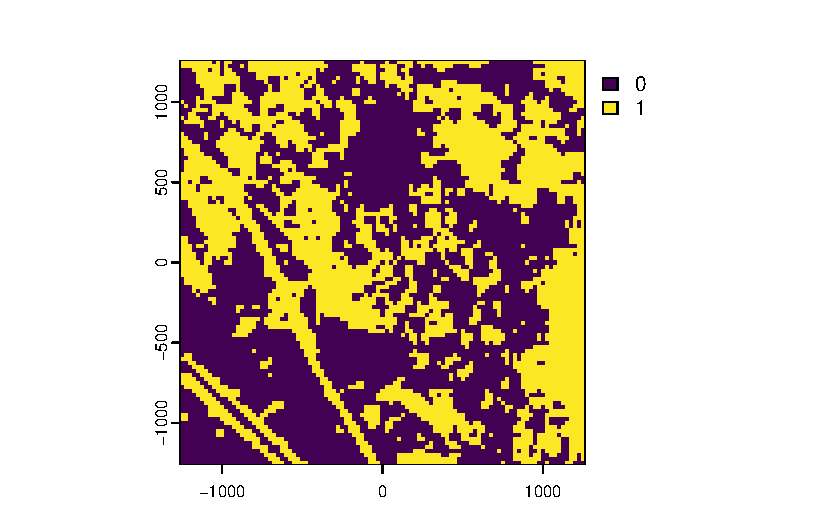
\includegraphics[keepaspectratio]{deepSSF_data_prep_id_files/figure-pdf/unnamed-chunk-12-6.pdf}}

\begin{Shaded}
\begin{Highlighting}[]
\CommentTok{\# Canopy cover}
\FunctionTok{walk}\NormalTok{(buffalo\_data\_covs}\SpecialCharTok{$}\NormalTok{canopy\_cover\_cent[}\DecValTok{1}\SpecialCharTok{:}\NormalTok{n\_plots], terra}\SpecialCharTok{::}\NormalTok{plot)}
\end{Highlighting}
\end{Shaded}

\pandocbounded{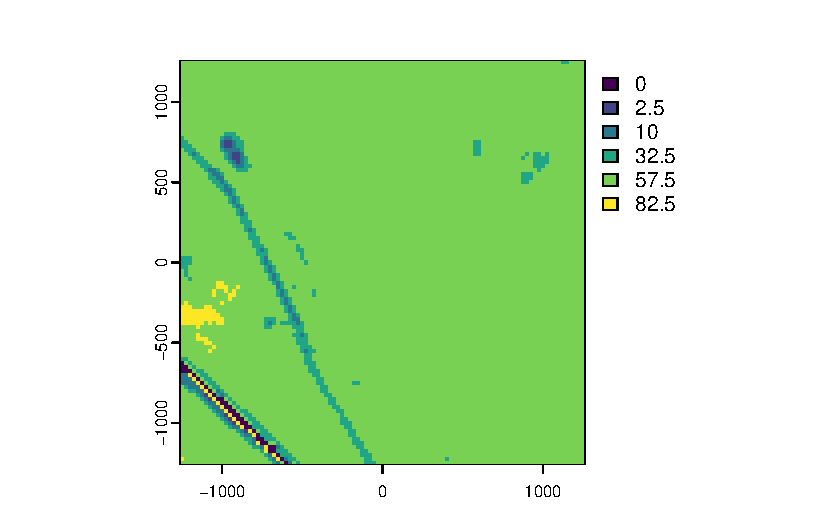
\includegraphics[keepaspectratio]{deepSSF_data_prep_id_files/figure-pdf/unnamed-chunk-12-7.pdf}}

\pandocbounded{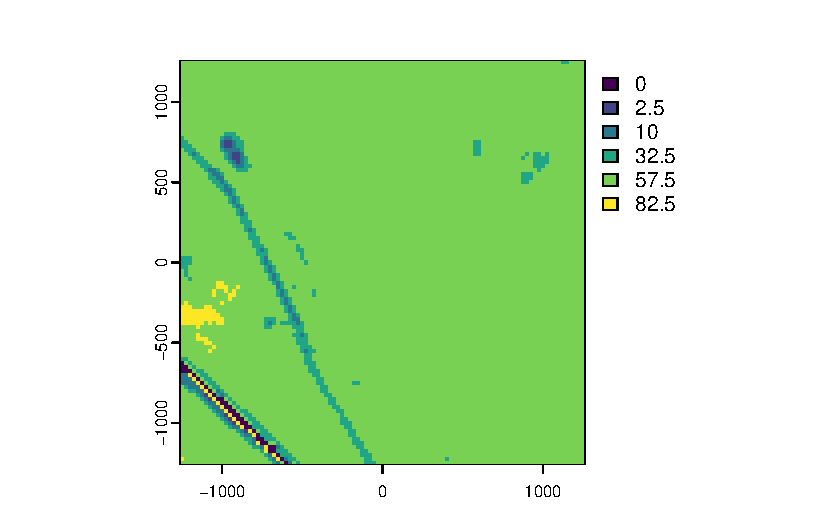
\includegraphics[keepaspectratio]{deepSSF_data_prep_id_files/figure-pdf/unnamed-chunk-12-8.pdf}}

\pandocbounded{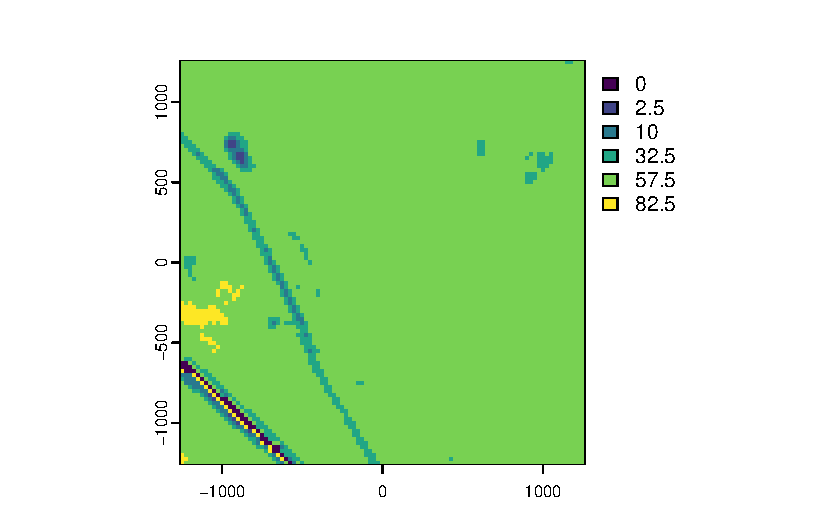
\includegraphics[keepaspectratio]{deepSSF_data_prep_id_files/figure-pdf/unnamed-chunk-12-9.pdf}}

\begin{Shaded}
\begin{Highlighting}[]
\CommentTok{\# Slope}
\FunctionTok{walk}\NormalTok{(buffalo\_data\_covs}\SpecialCharTok{$}\NormalTok{slope\_cent[}\DecValTok{1}\SpecialCharTok{:}\NormalTok{n\_plots], terra}\SpecialCharTok{::}\NormalTok{plot)}
\end{Highlighting}
\end{Shaded}

\pandocbounded{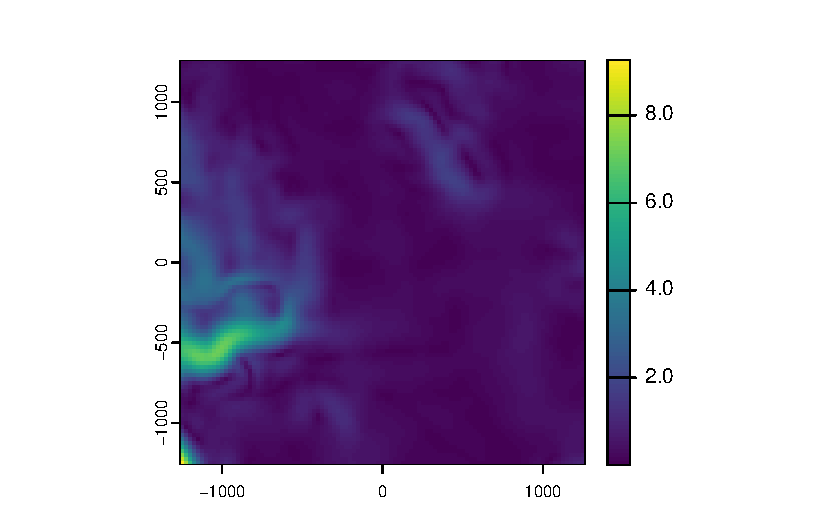
\includegraphics[keepaspectratio]{deepSSF_data_prep_id_files/figure-pdf/unnamed-chunk-12-10.pdf}}

\pandocbounded{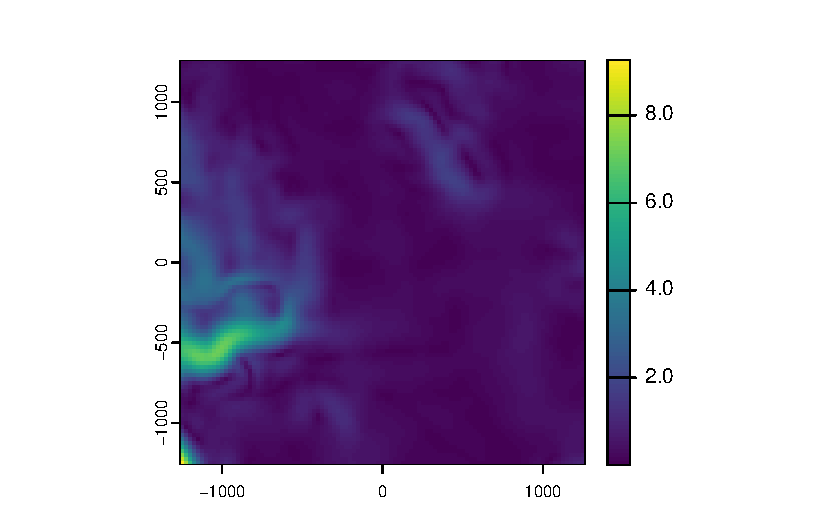
\includegraphics[keepaspectratio]{deepSSF_data_prep_id_files/figure-pdf/unnamed-chunk-12-11.pdf}}

\pandocbounded{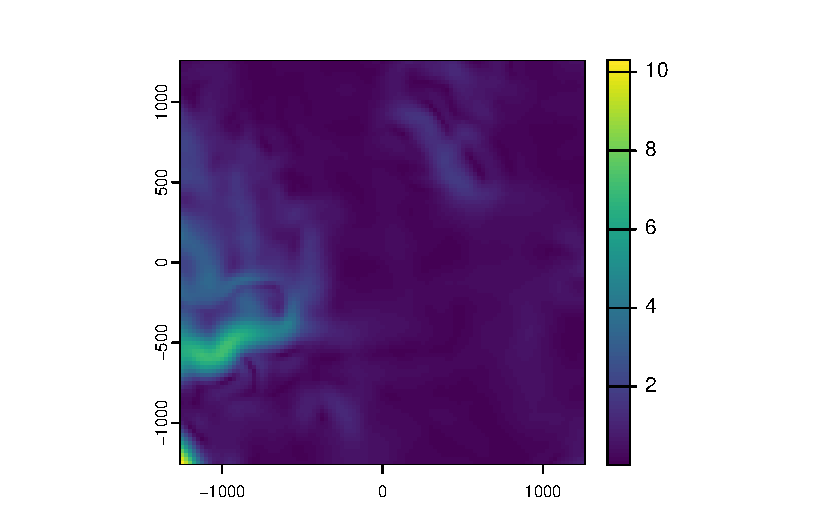
\includegraphics[keepaspectratio]{deepSSF_data_prep_id_files/figure-pdf/unnamed-chunk-12-12.pdf}}

\begin{Shaded}
\begin{Highlighting}[]
\CommentTok{\# Target (location of the next step)}
\FunctionTok{walk}\NormalTok{(buffalo\_data\_covs}\SpecialCharTok{$}\NormalTok{pres\_cent[}\DecValTok{1}\SpecialCharTok{:}\NormalTok{n\_plots], terra}\SpecialCharTok{::}\NormalTok{plot)}
\end{Highlighting}
\end{Shaded}

\pandocbounded{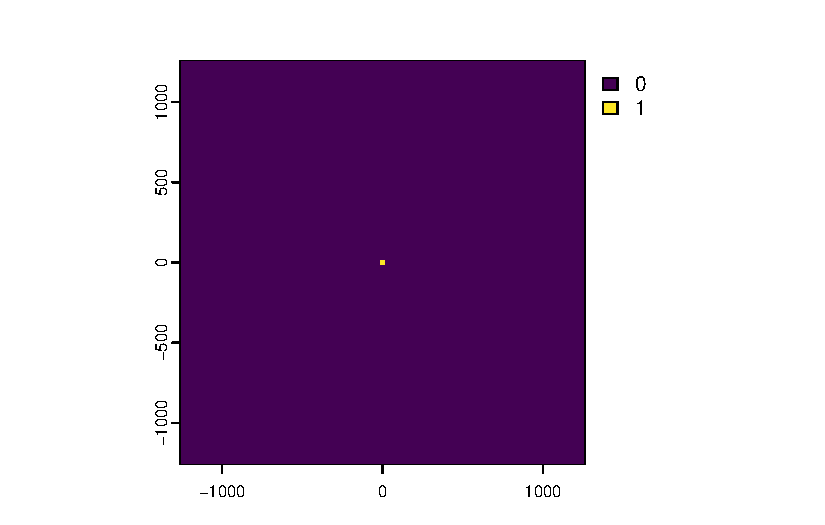
\includegraphics[keepaspectratio]{deepSSF_data_prep_id_files/figure-pdf/unnamed-chunk-12-13.pdf}}

\pandocbounded{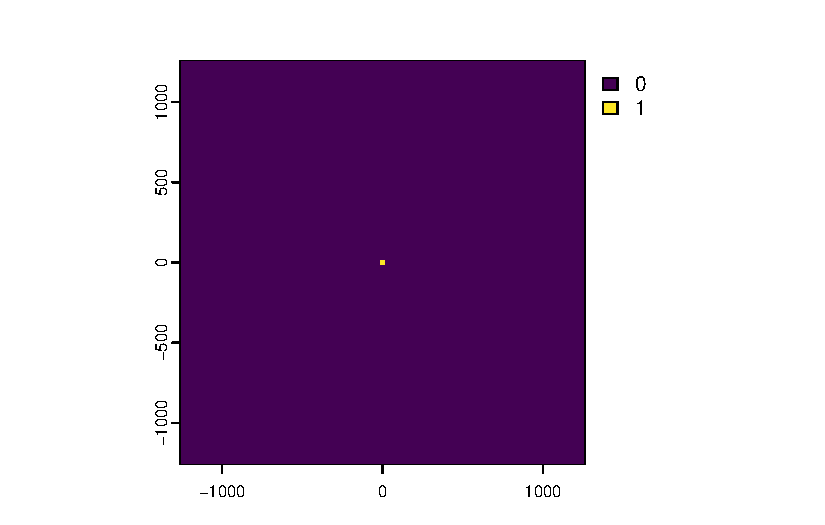
\includegraphics[keepaspectratio]{deepSSF_data_prep_id_files/figure-pdf/unnamed-chunk-12-14.pdf}}

\pandocbounded{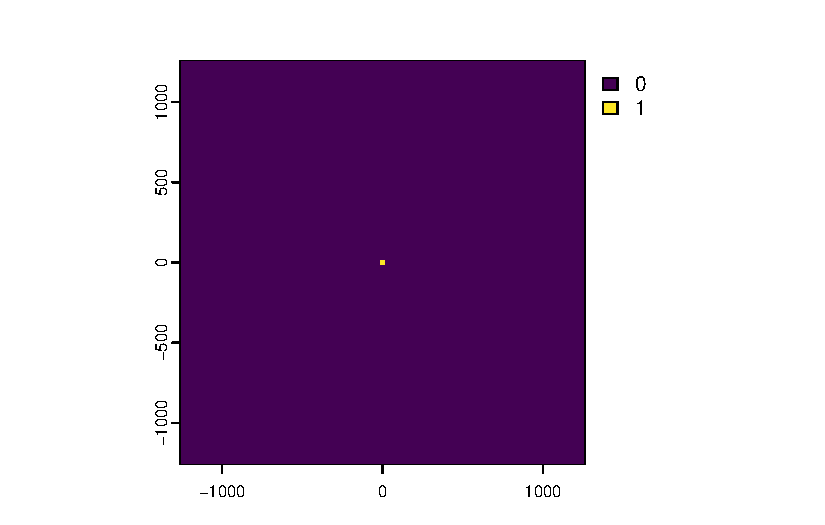
\includegraphics[keepaspectratio]{deepSSF_data_prep_id_files/figure-pdf/unnamed-chunk-12-15.pdf}}

\subsection{To save the object with all of the local
covariates}\label{to-save-the-object-with-all-of-the-local-covariates}

\begin{Shaded}
\begin{Highlighting}[]
\CommentTok{\# saveRDS(buffalo\_data\_covs, paste0("buffalo\_data\_id\_covs\_", Sys.Date(), ".rds"))}
\end{Highlighting}
\end{Shaded}

\subsection{To save some plots}\label{to-save-some-plots}

\begin{Shaded}
\begin{Highlighting}[]
\CommentTok{\# for(i in 1:n\_plots) \{}
\CommentTok{\#   png(filename = paste0("ndvi\_cent\_", i, ".png"),}
\CommentTok{\#       width = 150, height = 150, units = "mm", res = 600)}
\CommentTok{\#   terra::plot(buffalo\_data\_covs$ndvi\_cent[[i]])}
\CommentTok{\#   dev.off()}
\CommentTok{\# \}}
\CommentTok{\# }
\CommentTok{\# \# for the pres layers}
\CommentTok{\# for(i in 1:n\_plots) \{}
\CommentTok{\#   }
\CommentTok{\#   \# change the 0 values to NA}
\CommentTok{\#   layer \textless{}{-} buffalo\_data\_covs$pres\_cent[[i]]}
\CommentTok{\#   layer[layer == 0] \textless{}{-} 0.5}
\CommentTok{\#   }
\CommentTok{\#   ndvi\_layer \textless{}{-} buffalo\_data\_covs$ndvi\_cent[[i]]}
\CommentTok{\#   new\_layer \textless{}{-} layer*ndvi\_layer}
\CommentTok{\#   }
\CommentTok{\#   \# save the plot}
\CommentTok{\#   png(filename = paste0("pres\_cent\_", i, ".png"),}
\CommentTok{\#       width = 150, height = 150, units = "mm", res = 600)}
\CommentTok{\#   terra::plot(new\_layer)}
\CommentTok{\#   dev.off()}
\CommentTok{\# \}}
\CommentTok{\# }
\CommentTok{\# }
\CommentTok{\# \# other plots}
\CommentTok{\# }
\CommentTok{\# n\_plots \textless{}{-} 1}
\CommentTok{\# }
\CommentTok{\# for(i in 1:n\_plots) \{}
\CommentTok{\#   png(filename = paste0("veg\_herby\_cent\_", i, ".png"),}
\CommentTok{\#       width = 150, height = 150, units = "mm", res = 600)}
\CommentTok{\#   terra::plot(buffalo\_data\_covs$veg\_herby\_cent[[i]])}
\CommentTok{\#   dev.off()}
\CommentTok{\# \}}
\CommentTok{\# }
\CommentTok{\# for(i in 1:n\_plots) \{}
\CommentTok{\#   png(filename = paste0("canopy\_cover\_cent\_", i, ".png"),}
\CommentTok{\#       width = 150, height = 150, units = "mm", res = 600)}
\CommentTok{\#   terra::plot(buffalo\_data\_covs$canopy\_cover\_cent[[i]])}
\CommentTok{\#   dev.off()}
\CommentTok{\# \}}
\CommentTok{\# }
\CommentTok{\# for(i in 1:n\_plots) \{}
\CommentTok{\#   png(filename = paste0("slope\_cent\_", i, ".png"),}
\CommentTok{\#       width = 150, height = 150, units = "mm", res = 600)}
\CommentTok{\#   terra::plot(buffalo\_data\_covs$slope\_cent[[i]])}
\CommentTok{\#   dev.off()}
\CommentTok{\# \}}
\end{Highlighting}
\end{Shaded}

\subsection{Plot the step lengths and turning
angles}\label{plot-the-step-lengths-and-turning-angles}

\begin{Shaded}
\begin{Highlighting}[]
\CommentTok{\# plot step lengths}
\NormalTok{buffalo\_data\_covs }\SpecialCharTok{\%\textgreater{}\%} \FunctionTok{filter}\NormalTok{(sl }\SpecialCharTok{\textless{}} \DecValTok{2000}\NormalTok{) }\SpecialCharTok{\%\textgreater{}\%} \FunctionTok{ggplot}\NormalTok{() }\SpecialCharTok{+}
  \FunctionTok{geom\_density}\NormalTok{(}\FunctionTok{aes}\NormalTok{(}\AttributeTok{x =}\NormalTok{ sl), }
                 \AttributeTok{fill =} \StringTok{"skyblue"}\NormalTok{, }\AttributeTok{colour =} \StringTok{"skyblue"}\NormalTok{, }\AttributeTok{alpha =} \FloatTok{0.75}\NormalTok{) }\SpecialCharTok{+}
  \FunctionTok{scale\_x\_continuous}\NormalTok{(}\StringTok{"Step length (m)"}\NormalTok{) }\SpecialCharTok{+} \CommentTok{\#, limits = c({-}25, 1250)}
  \FunctionTok{scale\_y\_continuous}\NormalTok{(}\StringTok{"Density"}\NormalTok{) }\SpecialCharTok{+}
  \FunctionTok{ggtitle}\NormalTok{(}\StringTok{"Step lengths"}\NormalTok{) }\SpecialCharTok{+}
  \FunctionTok{theme\_classic}\NormalTok{()}
\end{Highlighting}
\end{Shaded}

\pandocbounded{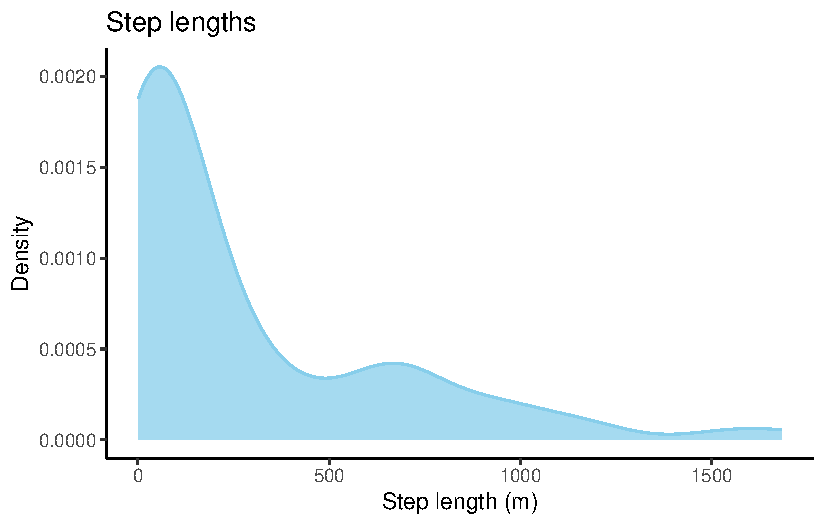
\includegraphics[keepaspectratio]{deepSSF_data_prep_id_files/figure-pdf/unnamed-chunk-15-1.pdf}}

\begin{Shaded}
\begin{Highlighting}[]
\CommentTok{\# ggsave("outputs/step\_length.png", height = 60, width = 120, units = "mm", dpi = 600)}


\CommentTok{\# plot turning angles}
\NormalTok{buffalo\_data\_covs }\SpecialCharTok{\%\textgreater{}\%} \FunctionTok{ggplot}\NormalTok{() }\SpecialCharTok{+}
  \FunctionTok{geom\_density}\NormalTok{(}\FunctionTok{aes}\NormalTok{(}\AttributeTok{x =}\NormalTok{ ta), }
                 \AttributeTok{fill =} \StringTok{"skyblue"}\NormalTok{, }\AttributeTok{colour =} \StringTok{"skyblue"}\NormalTok{, }\AttributeTok{alpha =} \FloatTok{0.75}\NormalTok{) }\SpecialCharTok{+}
  \FunctionTok{scale\_x\_continuous}\NormalTok{(}\StringTok{"Turning angle (radians)"}\NormalTok{, }
    \AttributeTok{breaks =} \FunctionTok{c}\NormalTok{(}\SpecialCharTok{{-}}\NormalTok{pi, }\SpecialCharTok{{-}}\NormalTok{pi}\SpecialCharTok{/}\DecValTok{2}\NormalTok{, }\DecValTok{0}\NormalTok{, pi}\SpecialCharTok{/}\DecValTok{2}\NormalTok{, pi),}
    \AttributeTok{labels =} \FunctionTok{c}\NormalTok{(}\FunctionTok{expression}\NormalTok{(}\SpecialCharTok{{-}}\NormalTok{pi), }\FunctionTok{expression}\NormalTok{(}\SpecialCharTok{{-}}\NormalTok{pi}\SpecialCharTok{/}\DecValTok{2}\NormalTok{), }\StringTok{"0"}\NormalTok{, }\FunctionTok{expression}\NormalTok{(pi}\SpecialCharTok{/}\DecValTok{2}\NormalTok{), }\FunctionTok{expression}\NormalTok{(pi))}
\NormalTok{  ) }\SpecialCharTok{+}
  \FunctionTok{scale\_y\_continuous}\NormalTok{(}\StringTok{"Density"}\NormalTok{) }\SpecialCharTok{+}
  \FunctionTok{ggtitle}\NormalTok{(}\StringTok{"Turning angles"}\NormalTok{) }\SpecialCharTok{+}
  \FunctionTok{theme\_classic}\NormalTok{()}
\end{Highlighting}
\end{Shaded}

\pandocbounded{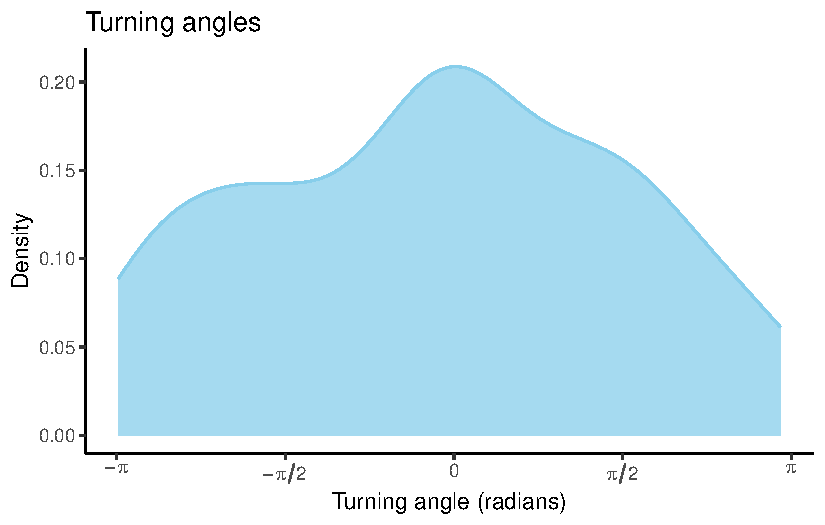
\includegraphics[keepaspectratio]{deepSSF_data_prep_id_files/figure-pdf/unnamed-chunk-15-2.pdf}}

\begin{Shaded}
\begin{Highlighting}[]
\CommentTok{\# ggsave("outputs/turning\_angle.png", height = 60, width = 120, units = "mm", dpi = 600)  }
\end{Highlighting}
\end{Shaded}





\end{document}
